\documentclass{beamer}
\usepackage[french]{babel}
\usepackage[utf8]{inputenc}
\usepackage[T1]{fontenc}
\usepackage{caption,subcaption,um}

\title[Introduction aux protocoles TCP/IP]{
  Réseau internet : une introduction aux protocoles de la famille TCP/IP}

\author[T. Di Giovanni et M. Beuret]{Thomas Di Giovanni et Maëlle Beuret}

\institute[Université de Montpellier]{
  Faculté des Sciences - Licence informatique\\
  Université de Montpellier}

\date[12 mai 2017]{12 mai 2017}

\begin{document}

\begin{frame}
  \titlepage
\end{frame}

\begin{frame}
  \frametitle{Table des matières}
  \tableofcontents
\end{frame}

% Introduction
\section{Introduction}

% Page 1
\begin{frame}
  \frametitle{Introduction}
    \begin{block}{Définition : protocole de communication}
        Ensemble de règles permettant de communiquer entre deux ordinateurs
    \end{block}
    \begin{itemize}
        \item TCP/IP (Transmission Control Protocol/Internet Protocol) : suite de protocoles réseau
        \item Également appelée famille des protocoles Internet
        \item Spécifications définies dans des documents du domaine public appelés RFC (Request For Comments)
        \item Développée durant les années 1970 et adoptée comme famille de protocoles standards pour ARPANET en 1983
    \end{itemize}
\end{frame}

% Chapitre 1
\section{Présentation générale}

\begin{frame}[allowframebreaks]
  \frametitle{Fonctionnement global}

    \begin{itemize}
      \item Utilise le modèle client/serveur
      \item Communication en point-à-point : d'un point (ou hôte) à un autre
      \item Fractionnement des messages en paquets
      \item Système d'adresses
      \item Acheminement des données sur le réseau
      \item Contrôle des erreurs
      
    \end{itemize}
    
    \begin{figure}
        \centering
        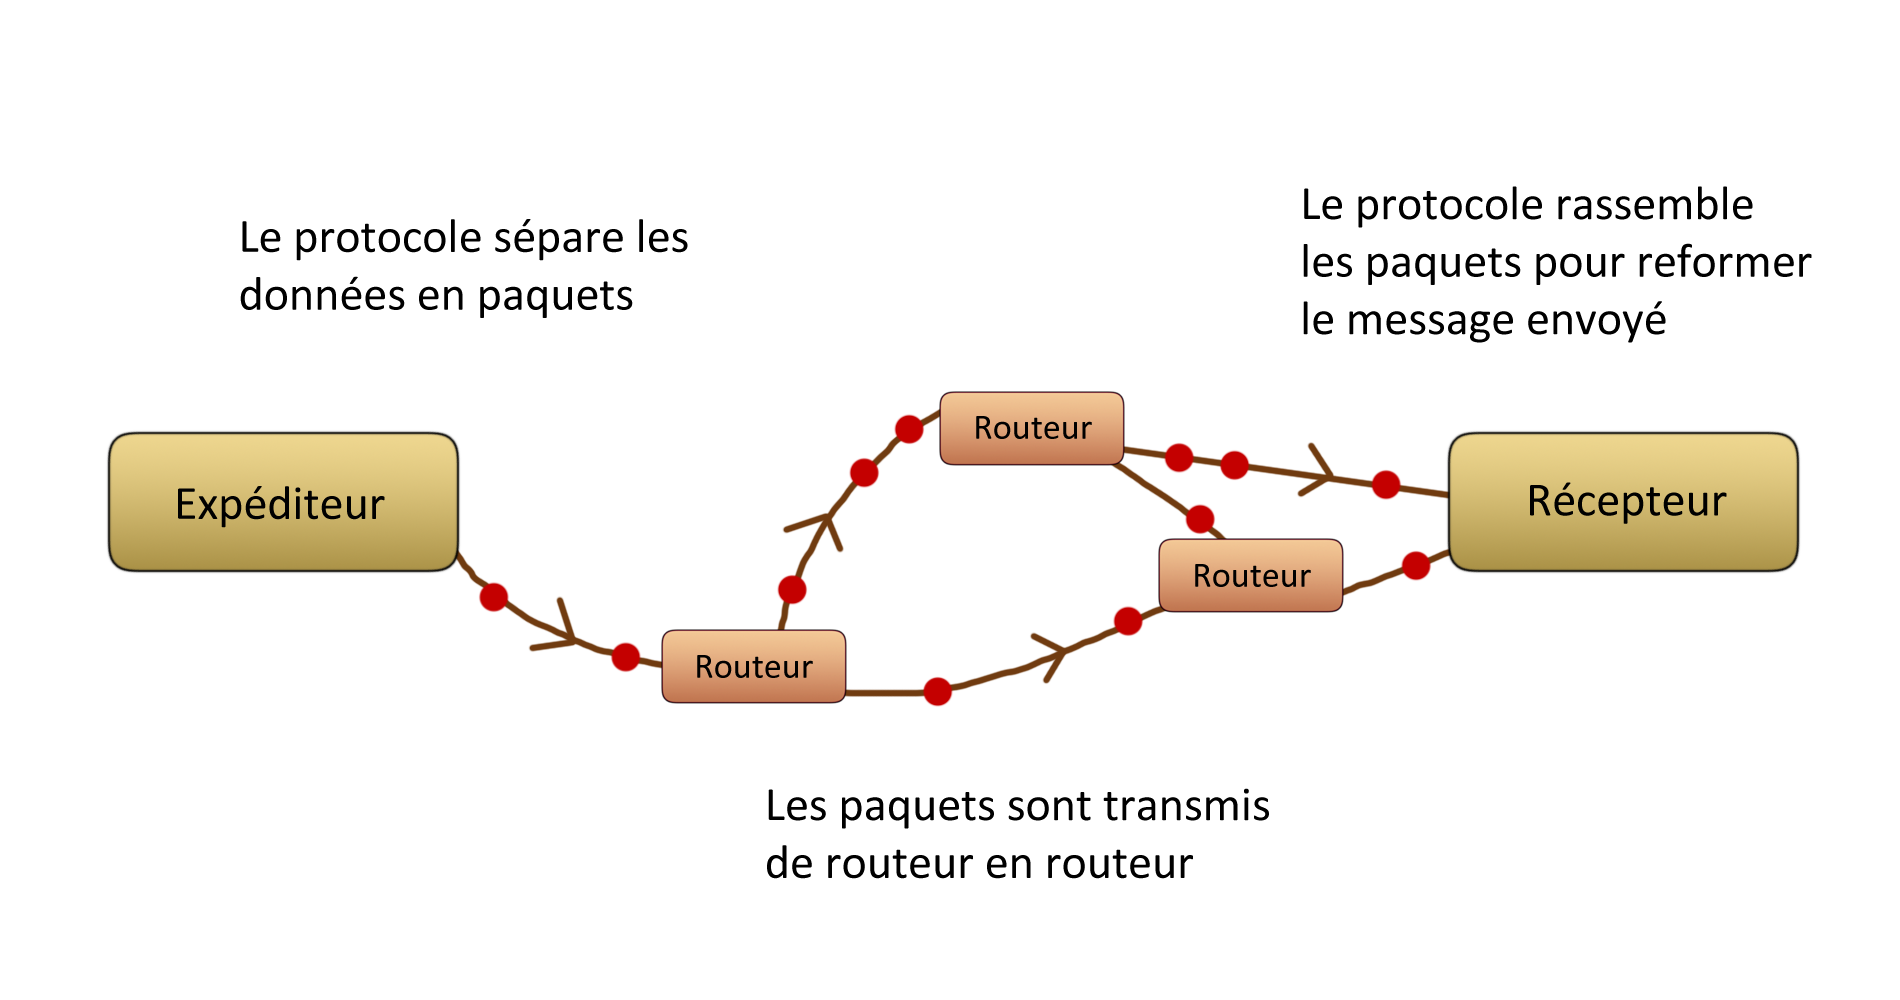
\includegraphics[scale=0.16]{TCP-IP}
        \caption{Fonctionnement de la transmission de données}
        \label{fig:my_label}
    \end{figure}
    
\end{frame}

\begin{frame}[allowframebreaks]
    \frametitle{Les protocoles du cœur de la suite}
        \begin{block}{Protocole IP}
            \begin{itemize}
                \item Détermine le destinataire grâce à l'adresse IP, le masque de sous-réseau et la passerelle par défaut
                \item Fragmente les datagrammes (paquets) au niveau des routeurs
                \item Assure l'acheminement des datagrammes à travers un réseau en empruntant le chemin le plus court (routage)
            \end{itemize}
        \end{block}
        
        \begin{block}{Protocole TCP}
            \begin{itemize}
                \item Permet de remettre en ordre les datagrammes en provenance du protocole IP
                \item Vérifie le flot de données (évite la saturation)
                \item Formate les données en segments pour que le protocole IP se charge du routage
                \item Multiplexe les données
                \item S'assure du bon fonctionnement de l'initialisation et de la fin d'une communication
            \end{itemize}
        \end{block}
        
        \begin{block}{Protocole UDP (User Datagram Protocol)}
            \begin{itemize}
                \item Permet d'assurer une transmission simple des données
                \item Ne garantit pas la bonne livraison des datagrammes à destination ni leur ordre d'arrivée
                \item Intégrité des données assurée par une somme de contrôle sur l'en-tête
                \item Utile pour une transmission rapide de petites quantités de données ou lorsque la perte d'un datagramme est moins problématique que le temps de transmission
            \end{itemize}
        \end{block}
    
\end{frame}

% Page 2
\begin{frame}[allowframebreaks]
  \frametitle{TCP/IP et OSI}

    \begin{itemize}
      \item Tous deux possèdent une architecture en couches
      \item Chaque couche TCP/IP correspond à une ou plusieurs couches OSI 
      \item OSI est en 7 couches et a rencontré moins de succès pratique 
      \item Ainsi, TCP/IP est devenu un modèle pratique et OSI un modèle théorique
    \end{itemize}
    \begin{figure}
        \centering
        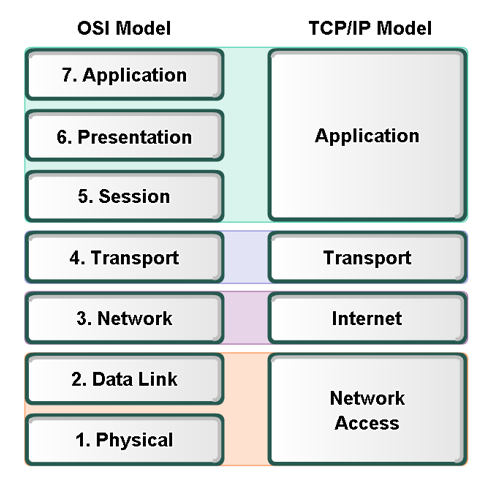
\includegraphics[scale=0.6]{1-OSI-TCPIP}
        \caption{Couches du modèle OSI et leur équivalent pour TCP/IP}
    \end{figure}

\end{frame}

% Chapitre 2
\section{Présentation détaillée des couches}

% Couches 1-2
\begin{frame}[allowframebreaks]
\frametitle{Couche "Accès réseau"}

Les rôles de cette couche :
  \begin{itemize}
    \item Le support de transmission des données
    \item La connexion des machines sur un réseau local
    \item La détection des erreurs à l'arrivée
  \end{itemize}
  \framebreak

Différents matériels utilisés, parmi les plus connus :
\begin{figure}[h]
    \begin{subfigure}[t]{0.33\textwidth}
        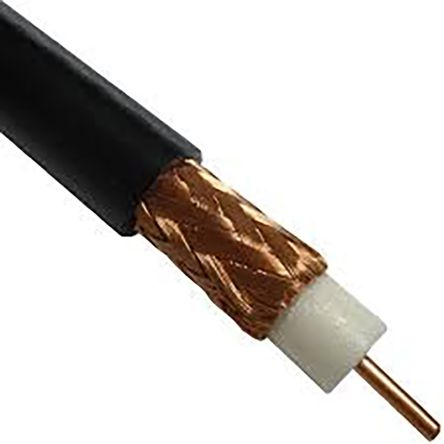
\includegraphics[scale=0.6]{2-Cable_coaxial}
        \caption{Câble coaxial} 
    \end{subfigure}%
    \begin{subfigure}[t]{0.33\textwidth}
        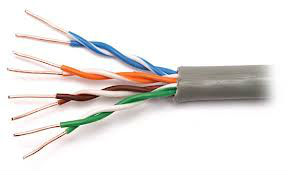
\includegraphics[scale=0.3]{2-Paire_torsadee}
        \caption{Paire torsadée}
    \end{subfigure}%
    \begin{subfigure}[t]{0.33\textwidth}
        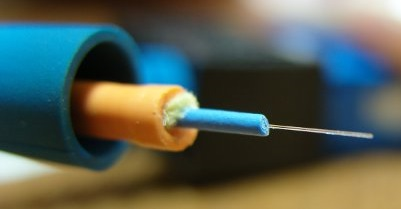
\includegraphics[scale=0.3]{2-Fibre_optique}
        \caption{Fibre optique}
    \end{subfigure}
\end{figure}
\framebreak
  
Trois topologies réseau principales :
\begin{figure}[h]
    \begin{subfigure}[t]{0.33\textwidth}
        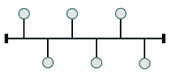
\includegraphics[scale=0.5]{2-Bus}
        \caption{En bus} 
    \end{subfigure}%
    \begin{subfigure}[t]{0.33\textwidth}
        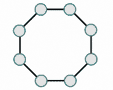
\includegraphics[scale=0.6]{2-Anneau}
        \caption{En anneau}
    \end{subfigure}%
    \begin{subfigure}[t]{0.33\textwidth}
        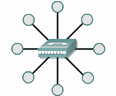
\includegraphics[scale=0.6]{2-Etoile}
        \caption{En étoile}
    \end{subfigure}
\end{figure}
\framebreak

    Pour communiquer, les machines utilisent une adresse MAC :
    \begin{itemize}
        \item L'adresse MAC est l'adresse d'une carte réseau.
        \item Chaque carte réseau a sa propre adresse, unique au monde.
        \item L'adresse MAC est écrite en hexadécimal, et codée sur 6 octets.
    \end{itemize}
    
    Il faut aussi un protocole particulier : Ethernet.
    \begin{itemize}
        \item Il n'est pas le seul protocole, mais il est de très loin le plus utilisé aujourd'hui.
        \item Le protocole va définir le format des messages (appelés trames) envoyés sur le réseau.
    \end{itemize}
    \framebreak
    
    \begin{block}{Le code de correction des erreurs (CRC)}
        Imaginons qu'une machine A envoie un message à une machine B.
        \begin{enumerate}
            \item Lors de l'envoi, A calcule le CRC et le met à la fin de la trame.
            \item B reçoit le message et fait le même calcul que A avec la trame reçue.
            \item B compare la valeur qu'elle a calculée avec la valeur que A avait calculée et mise à la fin de la trame.
            \item Si elles sont égales, la trame envoyée par A est identique à celle reçue par B. Sinon: erreur.
        \end{enumerate}
    \end{block}
    \framebreak
    
    \begin{figure}[h]
        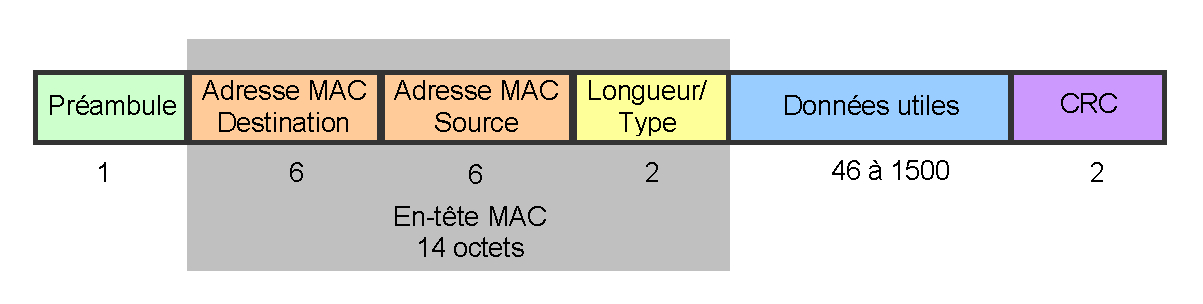
\includegraphics[scale=0.35]{2-Trame_Ethernet}
        \caption{Trame Ethernet}
    \end{figure}
    \framebreak
    
    Le commutateur (switch en anglais) est un boîtier sur lequel sont présentes plusieurs prises RJ45 femelles, ce qui permet de relier plusieurs machines entre elles.
    \begin{figure}[h]
        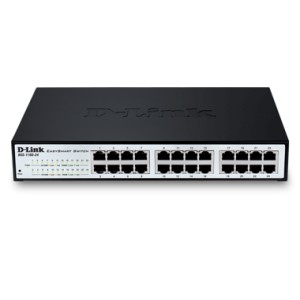
\includegraphics[scale=0.4]{2-Commutateur}
        \caption{Un commutateur}
    \end{figure}
    Il contient une table qui fait l'association entre un port et une adresse MAC. Cette table est appelée la table CAM.
    \begin{figure}[h]
        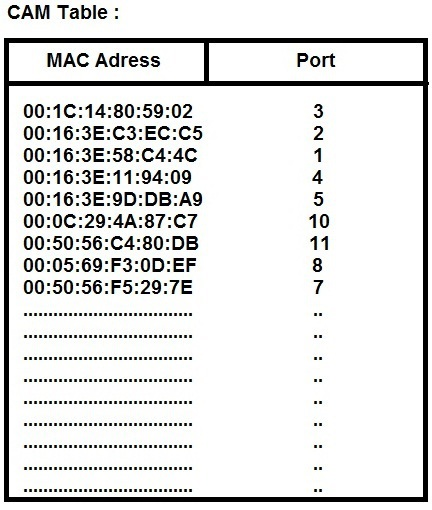
\includegraphics[scale=0.35]{2-Table_CAM}
        \caption{Une table CAM}
    \end{figure}
    
\end{frame}

% Couche 3
\begin{frame}[allowframebreaks]
  \frametitle{Couche "Internet"}

    Le rôle de cette couche est d'inter-connecter les réseaux : la connexion à une machine sur un autre réseau se fera à travers d'autres réseaux, de proche en proche. \newline
    
    Pour cela, on utilise l'adresse IP, qui est :
    \begin{itemize}
        \item L'adresse du réseau et de la machine
        \item Codée sur 32 bits ou 128 bits
    \end{itemize}
    
    On y ajoute un masque qui va indiquer quelle est la partie réseau de l'adresse (bits à 1), et quelle est la partie machine (bits à 0).
    \framebreak
    
    \begin{figure}[h]
        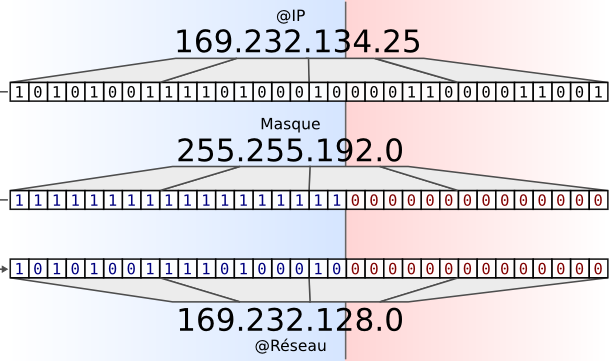
\includegraphics[scale=0.5]{2-Adresse_IP}
        \caption{Une adresse IP et son masque}
    \end{figure}
    \framebreak
    
    Une plage d'adresse est l'ensemble des adresses définies par l'association d'une adresse et d'un masque, de la plus petite adresse à la plus grande. \newline
    Nombre d'adresses dans un réseau =  $2^{NombreDe0DansLeMasque}$. \newline
    Deux adresses particulières dans la plage :
    \begin{itemize}
        \item La première est l'adresse du réseau
        \item La dernière est l'adresse de broadcast
    \end{itemize}
    \framebreak
    
    Autres protocoles de couche 3 :
    \begin{block}{Protocole ARP}
        Permet de connaître l'adresse physique d'une carte réseau correspondant à une adresse IP.
    \end{block}
    
    \begin{block}{Protocole ICMP}
        Permet de gérer les informations relatives aux erreurs aux machines connectées.
    \end{block}
    
\end{frame}

% Couche 4 
\begin{frame}[allowframebreaks]
  \frametitle{Couche "Transport"}

    Le rôle de cette couche est de permettre à des applications tournant sur des machines distantes de communiquer. \newline \newline
    Pour cela, elle utilise deux protocoles différents : TCP et UDP. \newline
    
    \begin{block}{Un identifiant, le port}
        Le port est l'adresse d'une application sur une machine. Il est codé en décimal sur deux octets.
    \end{block}
    
\end{frame}

% Couches 5-6-7
\begin{frame}[allowframebreaks]
  \frametitle{Couche "Application"}

    Elle contient les applications et programmes réseaux, ainsi que les protocoles qu'ils utilisent :
    \begin{itemize}
        \item Transfert de fichiers (FTP)
        \item Messagerie (SMTP)
        \item Connexion à distance sécurisée (SSH)
        \item World Wide Web (HTTP)
        \item etc...
    \end{itemize}
    
\end{frame}

% Conclusion
\section{Conclusion}

\begin{frame}
  \frametitle{Conclusion}

  La suite TCP/IP est :
  \begin{itemize}
      \item L'ensemble des protocoles utilisés pour le transfert des données sur Internet.
      \item L'implémentation du modèle OSI dans notre système d'exploitation.
      \item Représentée en 4 couches :
      \begin{enumerate}
          \item Accès réseau
          \item Internet
          \item Transport
          \item Application
      \end{enumerate}
  \end{itemize}
  
\end{frame}

\end{document}